% Options for packages loaded elsewhere
\PassOptionsToPackage{unicode}{hyperref}
\PassOptionsToPackage{hyphens}{url}
%
\documentclass[
]{book}
\usepackage{amsmath,amssymb}
\usepackage{lmodern}
\usepackage{ifxetex,ifluatex}
\ifnum 0\ifxetex 1\fi\ifluatex 1\fi=0 % if pdftex
  \usepackage[T1]{fontenc}
  \usepackage[utf8]{inputenc}
  \usepackage{textcomp} % provide euro and other symbols
\else % if luatex or xetex
  \usepackage{unicode-math}
  \defaultfontfeatures{Scale=MatchLowercase}
  \defaultfontfeatures[\rmfamily]{Ligatures=TeX,Scale=1}
\fi
% Use upquote if available, for straight quotes in verbatim environments
\IfFileExists{upquote.sty}{\usepackage{upquote}}{}
\IfFileExists{microtype.sty}{% use microtype if available
  \usepackage[]{microtype}
  \UseMicrotypeSet[protrusion]{basicmath} % disable protrusion for tt fonts
}{}
\makeatletter
\@ifundefined{KOMAClassName}{% if non-KOMA class
  \IfFileExists{parskip.sty}{%
    \usepackage{parskip}
  }{% else
    \setlength{\parindent}{0pt}
    \setlength{\parskip}{6pt plus 2pt minus 1pt}}
}{% if KOMA class
  \KOMAoptions{parskip=half}}
\makeatother
\usepackage{xcolor}
\IfFileExists{xurl.sty}{\usepackage{xurl}}{} % add URL line breaks if available
\IfFileExists{bookmark.sty}{\usepackage{bookmark}}{\usepackage{hyperref}}
\hypersetup{
  pdftitle={A Minimal Book Example},
  pdfauthor={John Doe},
  hidelinks,
  pdfcreator={LaTeX via pandoc}}
\urlstyle{same} % disable monospaced font for URLs
\usepackage{color}
\usepackage{fancyvrb}
\newcommand{\VerbBar}{|}
\newcommand{\VERB}{\Verb[commandchars=\\\{\}]}
\DefineVerbatimEnvironment{Highlighting}{Verbatim}{commandchars=\\\{\}}
% Add ',fontsize=\small' for more characters per line
\usepackage{framed}
\definecolor{shadecolor}{RGB}{248,248,248}
\newenvironment{Shaded}{\begin{snugshade}}{\end{snugshade}}
\newcommand{\AlertTok}[1]{\textcolor[rgb]{0.94,0.16,0.16}{#1}}
\newcommand{\AnnotationTok}[1]{\textcolor[rgb]{0.56,0.35,0.01}{\textbf{\textit{#1}}}}
\newcommand{\AttributeTok}[1]{\textcolor[rgb]{0.77,0.63,0.00}{#1}}
\newcommand{\BaseNTok}[1]{\textcolor[rgb]{0.00,0.00,0.81}{#1}}
\newcommand{\BuiltInTok}[1]{#1}
\newcommand{\CharTok}[1]{\textcolor[rgb]{0.31,0.60,0.02}{#1}}
\newcommand{\CommentTok}[1]{\textcolor[rgb]{0.56,0.35,0.01}{\textit{#1}}}
\newcommand{\CommentVarTok}[1]{\textcolor[rgb]{0.56,0.35,0.01}{\textbf{\textit{#1}}}}
\newcommand{\ConstantTok}[1]{\textcolor[rgb]{0.00,0.00,0.00}{#1}}
\newcommand{\ControlFlowTok}[1]{\textcolor[rgb]{0.13,0.29,0.53}{\textbf{#1}}}
\newcommand{\DataTypeTok}[1]{\textcolor[rgb]{0.13,0.29,0.53}{#1}}
\newcommand{\DecValTok}[1]{\textcolor[rgb]{0.00,0.00,0.81}{#1}}
\newcommand{\DocumentationTok}[1]{\textcolor[rgb]{0.56,0.35,0.01}{\textbf{\textit{#1}}}}
\newcommand{\ErrorTok}[1]{\textcolor[rgb]{0.64,0.00,0.00}{\textbf{#1}}}
\newcommand{\ExtensionTok}[1]{#1}
\newcommand{\FloatTok}[1]{\textcolor[rgb]{0.00,0.00,0.81}{#1}}
\newcommand{\FunctionTok}[1]{\textcolor[rgb]{0.00,0.00,0.00}{#1}}
\newcommand{\ImportTok}[1]{#1}
\newcommand{\InformationTok}[1]{\textcolor[rgb]{0.56,0.35,0.01}{\textbf{\textit{#1}}}}
\newcommand{\KeywordTok}[1]{\textcolor[rgb]{0.13,0.29,0.53}{\textbf{#1}}}
\newcommand{\NormalTok}[1]{#1}
\newcommand{\OperatorTok}[1]{\textcolor[rgb]{0.81,0.36,0.00}{\textbf{#1}}}
\newcommand{\OtherTok}[1]{\textcolor[rgb]{0.56,0.35,0.01}{#1}}
\newcommand{\PreprocessorTok}[1]{\textcolor[rgb]{0.56,0.35,0.01}{\textit{#1}}}
\newcommand{\RegionMarkerTok}[1]{#1}
\newcommand{\SpecialCharTok}[1]{\textcolor[rgb]{0.00,0.00,0.00}{#1}}
\newcommand{\SpecialStringTok}[1]{\textcolor[rgb]{0.31,0.60,0.02}{#1}}
\newcommand{\StringTok}[1]{\textcolor[rgb]{0.31,0.60,0.02}{#1}}
\newcommand{\VariableTok}[1]{\textcolor[rgb]{0.00,0.00,0.00}{#1}}
\newcommand{\VerbatimStringTok}[1]{\textcolor[rgb]{0.31,0.60,0.02}{#1}}
\newcommand{\WarningTok}[1]{\textcolor[rgb]{0.56,0.35,0.01}{\textbf{\textit{#1}}}}
\usepackage{longtable,booktabs,array}
\usepackage{calc} % for calculating minipage widths
% Correct order of tables after \paragraph or \subparagraph
\usepackage{etoolbox}
\makeatletter
\patchcmd\longtable{\par}{\if@noskipsec\mbox{}\fi\par}{}{}
\makeatother
% Allow footnotes in longtable head/foot
\IfFileExists{footnotehyper.sty}{\usepackage{footnotehyper}}{\usepackage{footnote}}
\makesavenoteenv{longtable}
\usepackage{graphicx}
\makeatletter
\def\maxwidth{\ifdim\Gin@nat@width>\linewidth\linewidth\else\Gin@nat@width\fi}
\def\maxheight{\ifdim\Gin@nat@height>\textheight\textheight\else\Gin@nat@height\fi}
\makeatother
% Scale images if necessary, so that they will not overflow the page
% margins by default, and it is still possible to overwrite the defaults
% using explicit options in \includegraphics[width, height, ...]{}
\setkeys{Gin}{width=\maxwidth,height=\maxheight,keepaspectratio}
% Set default figure placement to htbp
\makeatletter
\def\fps@figure{htbp}
\makeatother
\setlength{\emergencystretch}{3em} % prevent overfull lines
\providecommand{\tightlist}{%
  \setlength{\itemsep}{0pt}\setlength{\parskip}{0pt}}
\setcounter{secnumdepth}{5}
\usepackage{booktabs}
\usepackage{lscape}
\usepackage{longtable}
\usepackage{booktabs}
\usepackage{longtable}
\usepackage{array}
\usepackage{multirow}
\usepackage{wrapfig}
\usepackage{float}
\usepackage{colortbl}
\usepackage{pdflscape}
\usepackage{tabu}
\usepackage{threeparttable}
\usepackage{threeparttablex}
\usepackage[normalem]{ulem}
\usepackage{makecell}
\usepackage{xcolor}
\usepackage{fontspec}
\usepackage{multicol}
\usepackage{hhline}
\usepackage{hyperref}
\ifluatex
  \usepackage{selnolig}  % disable illegal ligatures
\fi
\usepackage[]{natbib}
\bibliographystyle{plainnat}

\title{A Minimal Book Example}
\author{John Doe}
\date{2021-12-01}

\begin{document}
\maketitle

{
\setcounter{tocdepth}{1}
\tableofcontents
}
\hypertarget{about}{%
\chapter{About}\label{about}}

This is a \emph{sample} book written in \textbf{Markdown}. You can use anything that Pandoc's Markdown supports; for example, a math equation \(a^2 + b^2 = c^2\).

\hypertarget{usage}{%
\section{Usage}\label{usage}}

Each \textbf{bookdown} chapter is an .Rmd file, and each .Rmd file can contain one (and only one) chapter. A chapter \emph{must} start with a first-level heading: \texttt{\#\ A\ good\ chapter}, and can contain one (and only one) first-level heading.

Use second-level and higher headings within chapters like: \texttt{\#\#\ A\ short\ section} or \texttt{\#\#\#\ An\ even\ shorter\ section}.

The \texttt{index.Rmd} file is required, and is also your first book chapter. It will be the homepage when you render the book.

\hypertarget{render-book}{%
\section{Render book}\label{render-book}}

You can render the HTML version of this example book without changing anything:

\begin{enumerate}
\def\labelenumi{\arabic{enumi}.}
\item
  Find the \textbf{Build} pane in the RStudio IDE, and
\item
  Click on \textbf{Build Book}, then select your output format, or select ``All formats'' if you'd like to use multiple formats from the same book source files.
\end{enumerate}

Or build the book from the R console:

\begin{Shaded}
\begin{Highlighting}[]
\NormalTok{bookdown}\SpecialCharTok{::}\FunctionTok{render\_book}\NormalTok{()}
\end{Highlighting}
\end{Shaded}

To render this example to PDF as a \texttt{bookdown::pdf\_book}, you'll need to install XeLaTeX. You are recommended to install TinyTeX (which includes XeLaTeX): \url{https://yihui.org/tinytex/}.

\hypertarget{preview-book}{%
\section{Preview book}\label{preview-book}}

As you work, you may start a local server to live preview this HTML book. This preview will update as you edit the book when you save individual .Rmd files. You can start the server in a work session by using the RStudio add-in ``Preview book'', or from the R console:

\begin{Shaded}
\begin{Highlighting}[]
\NormalTok{bookdown}\SpecialCharTok{::}\FunctionTok{serve\_book}\NormalTok{()}
\end{Highlighting}
\end{Shaded}

\hypertarget{reliabilitet}{%
\chapter{Reliabilitet}\label{reliabilitet}}

\hypertarget{introduksjon}{%
\section{Introduksjon}\label{introduksjon}}

Maksimalt oksygenopptak (VO2max) ble først beskrevet av Hill og Lupton i 1923, og kan defineres som kroppens evne til å ta opp og forbruke oksygen per tidsenhet \citep{bassett2000, hill1923}. Innen toppidrett måles ofte det maksimale oksygenopptaket for å måle utøverens kapasitet opp mot arbeidskravet i den spesifikke idretten, og VO2max kan i så måte også sees på som et mål på den aerobe effekten til utøveren \citep{bassett2000}. I Olympiatoppens testprotokoller benytter de flere definerte hjelpekriterier for å sikre at man faktisk har funnet deltakerens maksimale oksygenopptak \citep{tønnessen2017}. Følgende kriterier er beskrevet; platå i O2 er oppnådd, økning i ventilasjon med utflating av O2 verdi, RER-verdi over 1.10 (1.05 om gjennomført laktatprofiltest i forkant) og blodlaktat over 8 \citep{tønnessen2017}.

\hypertarget{metode}{%
\section{Metode}\label{metode}}

I forkant av testen målte alle deltakerne kroppsvekten i samme klær som ble brukt under testen, men ble bedt om å ta av seg skoene. Kroppsvekten som senere brukt i beregningen av maksimalt oksygenopptak (ml kg\textsuperscript{-1} min\textsuperscript{-1}) er kroppsvekten målt i forkant av test. For å sikre intern validitet ble deltakerne bedt om å avstå fra anstrengende fysisk aktivitet dagen før test, standardisere måltidet i forkant av test samt avstå fra inntak av koffein under de siste 12 timene før testen \citep{halperin2015} . Test 1 og Teat 2 ble gjennomført på samme tid på døgnet under standardiserte forhold.. Test 2 ble gjennomført 6 dager etter gjennomført Test 1. Det ble ikke kontrollert for fysisk aktivitet mellom testdagene.

Alle deltakerne gjennomførte en 10 minutter lang oppvarmingsprotokoll på tredemøllen (Woodway 4Front, Waukesha, USA), beskrevet for deltakerne i forkant av testen. Denne oppvarmingsprotokollen bestod av fem minutter på 11-13 i Borg 6-20 RPE skala \citep{borg1982}, etterfulgt av 2 drag med varighet på 1 minutt. Disse dragene var på samme hastighet og stigning som ved teststart, og ble adskilt med 30 sekunders pause hvor deltakerne sto i ro. De tre siste minuttetene av oppvarmingen var igjen begrenset til en intensitet mellom 11 og 12 på Borg skala. Etter gjennomført oppvarmingsprotokoll fikk deltakerne en pause på 2 minutter før testen begynte. Starthastighet for begge kjønn var satt til 8km/t, med stigning på 10.5\% og 5.5\% for henholdsvis menn og kvinner.

VO2max ble målt ved hjelp av en metabolsk analysator med miksekammer (vyntus CPX, mixing chamber (Vyntus CPX, Jaeger-CareFusion, UK). Forut for alle tester ble analysatoren gass- og volumkalibrert. Analysatoren ble stilt inn til å gjøre målinger hvert 30 sekunc, og VO2max ble kalkulert gjennom å bruke snittet av de to høyeste påfølgende målingene av O2. Det ble tatt en avgjørelse på at alle deltakerne underveis i testen mottok en høylytt verbal oppmuntring fra testleder, selv om dette vil ha en påvirkning på resultatene \citep{halperin2015}. Dette kan forsvares gjennom at man ønsket å bidra til at deltakerne faktisk gjennomførte testen til utmattelse, noe som også kan argumenteres for å være viktig å få valide resultater \citep[\citet{tønnessen2017}]{halperin2015}. Dette ble gjort både på Test 1 og Test 2. Alle deltakerne gjennomførte også begge testene med samme testleder og med samme personer til stede i rommet for å redusere konfundering \citep{halperin2015}.

For hvert medgåtte minutt av testen ble hastigheten på møllen økt med 1km/t, helt til utmattelse, hvor testen ble avsluttet. Deltakernes hjertefrekvens ble også registrert under hele testen. Når testen ble avsluttet ble deltakerne bedt om å rapportere opplevd anstrengelse ved hjelp av Borg-skala \citep{borg1982}. Maksimal hjertefrekvens under testen ble også registrert. Ett minutt etter avsluttet test ble hjertefrekvens registrert, og det ble målt og analysert blodlaktat (Biosen C-line, EKF Diagnostics, Barleben, Germany).

Det var 11 deltakere i studien, samtlige deltakere er studenter ved Høgskolen i Innlandet. Deskriptive data for disse deltakerne er vist i Tabell 1.

\hypertarget{resultater}{%
\section{Resultater}\label{resultater}}

Figur 1 viser utviklingen Test 1 til Test 2 fordelt på kjønn. Det typiske målefeilet (typical error, \citep{hopkins2000}) fra Test 1 til Test 2 er utregnet til å være 4.04\%. Det maksimale oksygenopptaket til de kvinnelige deltakerne spant seg fra 49.75 ml kg-1 min-1 til 54.50, mens det hos de mannlige deltakerne spant seg fra 49.50 ml kg-1 min-1 til 62.05 ml kg-1 min-1.

\begin{figure}
\centering
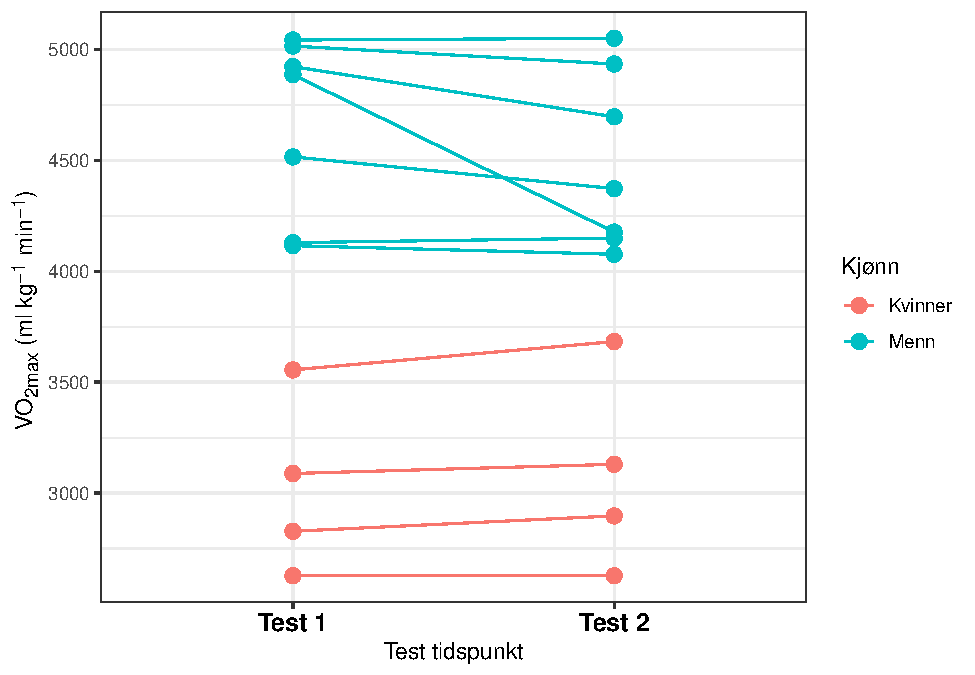
\includegraphics{_main_files/figure-latex/Figur-1.pdf}
\caption{\label{fig:Figur}VO2max ved Test 1 og Test 2.}
\end{figure}

\hypertarget{diskusjon}{%
\section{Diskusjon}\label{diskusjon}}

Det typiske målefeilet(TE) på 4.04\% kan også tyde på at enkelte av disse resultatene kan være utsatt for konfundering av ulik sort \citep{hopkins2000}. TE på 4.04\% kan derfor tenkes å være et bilde hvordan det kan se ut med få deltakere, med ulikt utgangspunkt, men også uten skikkelig standardisering av treningshverdagen i forkant av testene. Det kan også tenkes at med et varierende nivå hos deltagerne kan enkelte oppleve en treningseffekt av Test 1. Samtidig som andre kanskje ble slitne av å få en test inn i treningshverdagen.

Ettersom testing av maksimalt oksygenopptak er en test som gjennomføres til utmattelse, vil man kunne forvente en viss variasjon i testresultatene ettersom opplevd anstrengelse kan påvirkes av flere ulike variabler \citep{halperin2015}. For å redusere systematisk skjehvet i testresultat og målinger vil flere faktorer være nyttig å ta hensyn til under slik testing. Som nevnt i metoden vil standardisering av matinntak, koffeininntak, utstyr og tidspunkt for gjennomføring av test være med på å kunne sikre intern validitet i resultatene. Eksempler er deltakernes kjennskap til testen, verbal oppmuntring og personer tilstede under testen er andre faktorer som potensielt kan bidra til å påvirke resultatene. Felles for alle faktorer er at graden av påvirkning på resultatene muligens reduseres ved hjelp av en standardisert testprotokoll. Deltakerne - og testlederne, sin kjennskap til testen er en annen faktor som trolig påvirker resultatene i vårt prosjekt. I dette tilfellet fantes det enkelte deltakere som hadde gjennomført en liknende test flere ganger, og en kan da forvente en mindre grad av variasjon mellom resultatene på Test 1 og 2, sammenlignet med de deltakerne som gjennomførte testen for første gang på Test 1. Dette fordi kjennskapen og kunnskapen de tilegnet seg på Test 1, trolig spiller inn på testresultatene.

Grunnen til at vi snakker om typisk målefeil(TE) er at når vi ønsker å måle påvirkningen av trening på en gruppe individer er det viktig å kunne si noe om hva som er endring og hva som er støy (målefeil). Desto mindre støy en test innebærer jo bedre er målingen. Hva som danner denne variasjonen som kan observeres gjennom TE er multifaktorelt, men hoveddelen er som oftest biologisk \citep{hopkins2000}.

For å måle TE har vi brukt within subject deviation metoden. Denne metoden påvirkes ikke av at gjennomsnittet endrer seg fra test til test \citep{hopkins2000}. Data for målinger i VO2max fra fem sertifiserte Australske laboratorier fastslo ett gjennomsnitt på 2.2\% for TE \citep{halperin2015}. Data fra det Australske institutt for sport har også fastslått at en TE på omtrent 2\% er riktig for både maksimal og submaksimal O2 \citep{clark2007, robertson2010, saunders2009}. Dette indikerer at med godt kalibrert utstyr og med utøvere som er godt vant med testingen vil en TE på 2\% for det biologiske, og analytiske være riktig \citep{halperin2015}.

\hypertarget{referanser}{%
\section{Referanser}\label{referanser}}

\hypertarget{vitenskapsteori}{%
\chapter{Vitenskapsteori}\label{vitenskapsteori}}

\hypertarget{falsifikasjonisme}{%
\section{Falsifikasjonisme}\label{falsifikasjonisme}}

Poppers falsifiserbarhetskriterium dreier seg om differensieringen mellom vitenskapelige og uvitenskapelige teorier. Dette kriteriet går ut på at en teori må kunne falsifiseres for at den skal kunne betraktes som en vitenskapelig teori. På samme måte som teorier som ikke kunne falsifiseres da i den andre enden må betraktes som uvitenskapelige teorier(Karl R Popper, 1972). Det kan argumenteres for at et slikt kriterium løser demarkasjonsproblemet og gjør det mulig å unngå induksjonsproblemet i vitenskapsfilosofi, som det er mange meninger om(Karl R Popper, 1972; Vickers, 2006)

Hovedproblemet som falsifiserbarhetskriteriumet gir svar på er nok allikevel demarkasjonsproblemet. Demarkasjonsproblemet baserer seg på utfordringen mellom å skille mellom vitenskapelige og uvitenskapelige teorier(Karl R Popper, 1972). Popper argumenterer for at det er tilstrekkelig å skille mellom en vitenskapelig og en uvitenskapelig teori, hvor på den andre siden Okasha og andre vitenskapsfilosofier argumenterer for at dette problemet ikke i seg selv er avgjørende å løse(Okasha, 2002). Grunnen til dette er at de mener det ikke finnes en tydelig avgrensning mellom hvilke teorier som kan betraktes som vitenskapelige og uvitenskapelige, og det på en annen side er viktigere å skille mellom teorier som har blitt bekreftet flere ganger, og teorier som ikke er bekreftet. De ønsker altså heller å skille mellom hvor godt og hvor dårlig en vitenskapelig teori er bekreftet, fremfor å dedikere avgrensningen til om noe er vitenskapelig eller uvitenskapelig(Karl R Popper, 1972; Okasha, 2002; Vickers, 2006)

Sammen med å foreslå fasifiserbarhetskriteriumet som en løsning på demarkasjonsproblemet argumenterte Popper for at vi på denne måten også kan unngå induksjonsproblemet(Karl R Popper, 1972; Okasha, 2002; Vickers, 2006). Induksjonsproblemet dreier seg i motsetning til demarkasjonsproblemet mer om vitenskapelige argument. Det dreier seg i stor grad om det vil være mulig trekke slutninger om fremtiden basert på observasjoner vi gjør i dag(4. KvantMet2021 Vitenskapelige argument.pdf: IDR4000-1 21H Kvantitativ metode og statistikk, u.å.; Vickers, 2006). Popper mente at alle vitenskapelige argument er deduksjoner som igjen falsifiserer en vitenskapelig teori. Gjennom deduksjon kan man derfor falsifisere en teori, før denne forkastes og erstattes med en ny. Kritikken rundt å bruke induksjon som vitenskapelige argument er derfor ikke lenger aktuell, ettersom man gjennom deduksjon og falsifikasjon enkelt kan unngå å bruke induksjon i vitenskapen(Karl R Popper, 1972). Der hvor andre vitenskapsfilosofer er opptatt av å bekrefte teorier, ønsket Popper heller å falsifisere og erstatte disse. Dette gjenspeiles videre i uenigheten omkring skillet mellom vitenskapelige og uvitenskapelige teorier, der spesielt Popper var opptatt av at det skulle være et markert skille påsto den andre leiren at det ikke finnes et særlig skarpt skille. Popper mente altså gjennom sin falsifikasjonisme at en vitenskapelig teori bare kunne bli falsifisert, mens andre vitenskapsfilosofer argumenterte for at den viktigste forskjellen lå i hvor godt eller dårlig bekreftet en teori var.

\hypertarget{hd-metoden-og-abduksjon}{%
\section{HD-metoden og abduksjon}\label{hd-metoden-og-abduksjon}}

Strukturen på et bekreftende vitenskapelig argument er i følge den hypotetisk deduktive metoden slik at man legger opp deduktive argument fra teorien til dataen, gjennom å dedusere data fra teorien.(4. KvantMet2021 Vitenskapelige argument.pdf: IDR4000-1 21H Kvantitativ metode og statistikk, u.å.). Man benytter teorien for å skape deduktive argumenter for hvordan dataen induktivt skal bekrefte teorien. Gjennom å dedusere data fra teorien vil det bety at teorien kan bekreftes. Men bare til en viss grad, dette er også grunnen til at mange derfor påstår at det bekreftende vitenskapelige argumentet faktisk er en induktiv bekreftelse snarere enn en deduktiv bekreftelse.

I den hypotetisk deduktive metoden formuleres en teori eller en hypotese før det dannes empiriske konsekvenser fra disse(4. KvantMet2021 Vitenskapelige argument.pdf: IDR4000-1 21H Kvantitativ metode og statistikk, u.å.; 5. KvantMet2021 Abduksjon og sannsynlighet.pdf: IDR4000-1 21H Kvantitativ metode og statistikk, u.å.). Gjennom å gjenta observasjoner eller eksperimenter for å teste og undersøke de empiriske konsekvensene, vil man kunne oppnå en bekreftelse eller avkreftelse av hypotesen eller teorien(Hempel, Carl G, 1966). Denne prosessen mener Hempel er en induktiv prosess, ettersom det ved en induktiv bekreftelse av teorien gjennom observasjon av empiriske konsekvenser. Teorien er bekreftet til en viss grad. Derimot er konsekvensene vi tester deduktivt utledet fra teorien, og det er nettopp disse deduktive konsekvensene vi tester for å induktivt kunne bekrefte teorien eller hypotesen vi undersøker.

Kort fortalt kan man den hypotetisk deduktive metoden beskrives på en måte der man ut ifra en idé eller teori sammenligner faktiske observasjoner med de forventede observasjonene teorien legger grunnlag for.

Hempel argumenterer for at gjennom å ta utgangspunkt i teorien, fremfor eksempelvis å ta utgangspunkt i observasjoner kunne utlede vitenskapelige argument på en mye mer effektiv måte(Hempel, Carl G, 1966). Kanskje spesielt sammenlignet med Bacons naive induktivisme(4. KvantMet2021 Vitenskapelige argument.pdf: IDR4000-1 21H Kvantitativ metode og statistikk, u.å.) Sammenligner man Hempels hypotetisk deduktive metode med Poppers falsifikasjonisme, ser man en tydelig retning mot bekreftelse i Hempels metode, kontra avkreftelse i Poppers metode(Hempel, Carl G, 1966; Karl R Popper, 1972). Der Hempel ønsket å argumentere for, og å bekrefte ulike teorier i større eller mindre grad, ønsket popper å kunne skille tydelig mellom de vitenskapelige og ikke vitenskapelige teoriene, og helle falsifisere og argumentere mot teorier.

Sammenligner man den hypotetisk deduktive metoden med abduksjon så er det mange likheter(4. KvantMet2021 Vitenskapelige argument.pdf: IDR4000-1 21H Kvantitativ metode og statistikk, u.å.). I abduksjon vil man på samme måte som i den hypotetisk deduktive metoden ta utgangspunkt i en teori som man deretter danner grunnlag for å forklare forventede observasjoner, før man sammenligner de faktiske observasjonene med forventningen for å kunne gjøre en induktiv bekreftelse på teorien. I abduksjon forsøker man derimot i større grad å unngå deduksjon, noe som kan argumenteres for å være en utfordring i den hypotetisk deduktive metoden(5. KvantMet2021 Abduksjon og sannsynlighet.pdf: IDR4000-1 21H Kvantitativ metode og statistikk, u.å.). Utfordringen ligger i argumentasjonen om at dataen og de forventede observasjonene man skal bruke til å induktivt bekrefte teorien ikke kan blir dedusert fra teorien. Her prøver heller abduksjonen å utlede empiriske konsekvenser induktiv fra teorien, for så å induktiv bekrefte teorien på nytt. Man angriper altså teorien og de empiriske konsekvensene på en noe mer logisk måte, gjennom å si at teorien vill gi en god forklaring på de relevante dataene vi sitter med, og at man velger den teorien som gir den mest logiske forklaringen på teorien. De empiriske konsekvensene man da danner, vil kunne observeres og etterprøves i eksperiment, for så å muligens kunne gi en induktiv bekreftelse av teorien og fortelle oss at teorien stemmer, til en viss grad. Der hvor den hypotetisk deduktive metoden låser seg til én enkelt hypotese, kan en i abduksjonen benytte seg av flere ulike teorier. De ulike teoriene kan sammenlignes så lenge de kan gi en forklaring på det samme fenomenet, og deretter vil man velger den teorien som gir den beste forklaringen på teorien(5. KvantMet2021 Abduksjon og sannsynlighet.pdf: IDR4000-1 21H Kvantitativ metode og statistikk, u.å.). Abduksjonen vil for mange kunne oppleves som en større grad av subjektivitet, for hva er det egentlig som kan avgjøre om en teori gir en bedre forklaring på et fenomen enn ett annet, så lenge begge forklarer fenomenet? Videre kan abduksjonen fremstå som en mer effektiv vitenskapelig metode sammenlignet med den hypotetisk deduktive metoden, ettersom den hypotetisk deduktive metoden trolig dekker færre teorier enn hva abduksjon gjør. Til en viss grad kan det da argumenteres for at abduksjon som en vitenskapelig metode klarer å prøve ut flere teorier, og skille ut de som gir en dårligere forklaring på teorien, før man leter etter en måte å induktivt bekrefte denne teorien på.

\hypertarget{replikasjonskrisen}{%
\section{Replikasjonskrisen}\label{replikasjonskrisen}}

Replikasjonskrisen i forskningen oppstår i forbindelse med at flere godt bekreftede eksperimentale resultater i ettertid blir motbevist og stilt spørsmålstegn ved etter at andre forskere har prøvd å replisere de orginale studiene(Bird, 2020). Flere og flere forskningsfunn blir argumentert for at det falske, eller feil analysert (Dalen-Lorentsen et al., 2020; Ioannidis, 2005). En vanlig forklaring bak replikasjonskrisen er ofte dårlig forskningskvalitet. Dårlig forskningspraksis, publikasjonsbias, dårlige insentiver og forskningsjuks(Fanelli, 2009; Joober et al., 2012). Bird forsøker å forklare og argumentere for hvorfor den høye andelen av mislykkede replikasjoner er samsvarende med god forskningspraksis og forskning på høyt nivå(Bird, 2020). Han argumenterer for at dette er et forventet utfall innen forskningsmiljøer som produserer en stor andel av falske hypoteser i forkant av testing. En slik fremgangsmåte vil føre til -- sammen med en akseptert p-verdi og antatt insidens av type-1 feil på 5\%. Disse tingene argumenterer han igjen at skyldes basefrekvensfeilen, og legger dette til grunn som en viktig årsak til den manglende evnen til å replisere studier innenfor spesielt sosialpsykologi og klinisk medisin(Bird, 2020).

Bird forklarer replikasjonskrisen gjennom at basefrekvensefeilen antakelig vil oppstå når man gjør en konklusjon ut fra observasjoner eller eksperiment som påvirkes av sannsynligheten for at en bestem hendelse av et generelt fenomen. Et slik generell fenomen kan for eksempel være om en gitt person i en gitt befolkning utvikler en bestemt form for sykdom eller ikke. Feilen Bird snakker om vil oppstår når man kun legger vekt på et enkelt bevis som skal forklare og underbygge hendelsen. Hvor vanlig eller hvor sjelden denne hendelsen er i utgangpsunktet, vil oftere neglisjeres, og man trekker derfor skjeve slutninger. Konklusjonene vil da ofte være at en faktor eller et bevis har en tydelig samvariasjon med undersøkelsene, men man glemmer at fenomenet i seg selv er veldig sjeldent. Eksempelvis når man undersøker styrken til en klinisk test, hvor sensitiviteten og spesifisiteten på en test blir målt til å være veldig god i de tilfellene hvor fenomenet faktisk oppstår, men når dette sammenlignes på populasjonsnivå så overser man sannsynligheten for at fenomenet oppstår i seg selv, og sannsynligheten for at testen faktisk vil finne det fenomenet eller resultatet som undersøkes påvirkes da i veldig stor grad(6. KvantMet2021 Sannsynlighet og replikasjonskrisen.pdf: IDR4000-1 21H Kvantitativ metode og statistikk, u.å.)

Selv om replikasjonskrisen trolig til en viss grad kan forklares av Birds argumenter, skal man ikke se langt tilbake i historien for å finne eksempler på andre forklaringer på krisen(Fanelli, 2009; Joober et al., 2012). Publikasjonsbias i seg selv har vært et emne som har fått mye oppmerksomhet de siste årene, samtidig som det er flere og flere eksempler på økende grad av artikler som trekkes tilbake på bakgrunn av nettopp bias, tvilsom forskningspraksis, juks eller svindel(Amos, 2014; Figure 2, u.å.). Økonomi og konkurranse mellom ulike forskningsinstitutt spiller trolig også inn, og man ser tidvis eksempler på dette også spesielt innen idrettsmedisin og idrettsvitenskap, der ofte ulike konkurrerende forskningsmiljøer ser ut til å ha en tendens til å gå etter hverandres forskning i sømmene(Dalen-Lorentsen et al., 2020; Hulin et al., 2016; Impellizzeri et al., 2021; van der Horst et al., 2014).

\hypertarget{studiedesign}{%
\chapter{Studiedesign}\label{studiedesign}}

\hypertarget{formuxe5l}{%
\section{Formål}\label{formuxe5l}}

Forfatterne i samtlige studier inkludert i denne oppgaven ønsker å bidra til økt kunnskap som kan være med å løse den økende utfordringen med hamstringsskader i idretten, ettersom denne utfordringen har store konsekvenser for både prestasjon og økonomi \citep{ekstrand2011, hickey2014, eirale2013, hickey2020, askling2014, hamilton2015, ahamid2014, askling2013}. Forfatterne ønsker å bidra til en økt kunnskap gjennom å formulere ulike spørsmål og sammenligningsgrunnlag. Alle studier har som formål å sammenligne to eller flere ulike rehabiliteringsprotokoller for å se hvilken av disse som har best effekt på tid til retur til idrett. Mer spesifikt ønsker tre av studiene å sammenligne hvilken effekt to ulike typer aktive rehabiliteringsprotokoller har på tiden det tar for å returnere til idrett etter en akutt hamstringsskade\citep[\citet{askling2013}, \citet{hickey2020}]{askling2014}. De to andre studiene forsøker å se hvilken effekt injeksjoner av Platelet-Rich-Plasma (PRP) har på rehabiliteringen av en hamstringsskade når det kombineres med aktiv rehabilitering, målt gjennom tid til retur til idrett\citep{ahamid2014, hamilton2015}.

Den røde tråden i disse artiklene finner vi igjen i utgangspunktet samtlige forfattere har i den tydelige byrden hamstringsskader har på prestasjon og økonomi i toppidretten\citep{ekstrand2011, hickey2014, eirale2013}. Videre vil kunnskapen vi allerede har, og dagens praksis omkring rehabiliteringen av hamstringsskader være med å påvirke retningen på disse studiene \citep{brooks2006, horst2017, opar2012, podlog2014}. Økt kunnskap leder ofte til økt nysgjerrighet, og tiltak for å ytterlige optimalisere denne rehabiliteringsprosessen vil potensielt kunne gi tydelige fortrinn i toppidretten på flere ulike måter, hvor prestasjon og økonomi skiller seg ut som de to store.

\hypertarget{metodisk-sammenligning}{%
\section{Metodisk sammenligning}\label{metodisk-sammenligning}}

Detaljert karakteristikk i metoden til de ulike studiene inkludert finnes i Tabell 1.

Alle de fem inkluderte artiklene er designet som randomiserte kontrollerte studier(RCT)\citep{askling2014, askling2013, hickey2020, ahamid2014, hamilton2015}.En RCT er et forskningsstudie som sammenligner to eller flere forskjellige grupper\citep[s 137-139.]{hulley2013}. Ofte mottar en av gruppene en form for intervensjon man ønsker å undersøke, samtidig som den andre gruppen mottar enten ingen intervensjon, eller en annen form for intervensjon. Gruppen som ikke mottar en intervensjon, eller eventuelt en placebointervensjon, kalles ofte kontrollgruppe. Intervensjonen varierer fra fagfelt til fagfelt, men er ofte en form for behandling, trening, medisinering eller lignende. Målet med en RCT er å sammenligne utfallet en intervensjon har på én gruppe, opp mot utfallet i en annen gruppe som enten mottok ingen intervensjon eller en annen type intervensjon. På denne måten ønsker man i gjennom et RCT-design å trekke slutninger om sammenhenger mellom årsak og effekt\citep[s. 121]{hulley2017}. I slike studier er ofte blinding av deltakere og forskningspersoner, samt randomisering av gruppene to hjørnesteiner for å i større grad kunne oppnå disse målene om inferens\citep[s.138-140]{hulley2017}.

Dette er et studiedesign som ligger høyt på evidenspyramiden, og i mindre grad er utsatt for bias og konfundering sammenlignet med andre type design som for eksempel case-control design og cohortdesign\citep[s.109-110]{hulley2017}. Samtidig er dette også et studiedesign som er mer kostbart og tidkrevende, i tillegg til at studiedesignet muligens krever mer detaljplanlegging og omfattende arbeid rundt speiselt randomisering og blinding \citep[s.139-141]{hulley2017}. Det er også enkelte fagfelt eller forskningsområder der en blinding av deltakerne, en placebo-kontroll, eller blinding av forskningspersoner ikke alltid er mulig å gjennomføre, slik som for eksempel trening, manuell behandling, ortopedi, psykiatri eller lignende. Derfor vil man ofte kunne se sammenligninger av to intervensjoner, fremfor sammenligning mot en kontroll\citep[s.137-139]{hulley2017}.

Deltakerne i studiene er hentet fra en populasjon av voksne idrettsutøvere med akutte hamstringsskader. Tretten ulike idretter er representert, med fotball og friidrett som de to største. Utvalgsstørrelsen varierte fra 24 til 90, med et snitt på 62 deltakere over de fem studiene. Totalt var det 308 deltakere, kjønnsfordelingen var omtrent 9\% kvinner og 91\% menn. To av studiene hadde kun mannlige deltakere \citep{hickey2020, hamilton2015}.Tre av studiene hadde på forhånd gjort en utregning av ønsket utvalgsstørrelse for en statistisk styrke på 80\% \citep{hickey2020, ahamid2014, hamilton2015}.

Statistisk styrke er et mål på sannsynligheten forskeren har for å finne en statistisk signifikans forskjell dersom det finnes en reell forskjell i populasjonon\citep[\citet{turner2018}]{jones2004}. Det vil si at dersom forfatterne har klart å oppnå den ønskede utvalgsstørrelsen, vil de ha 80\% sannsynlighet for å oppdage en statistisk signifikant forskjell mellom de ulike rehabiliteringsmetodene de undersøker, dersom den effekten er reell. Dette påvirkes også av angitt p-verdi, som sier oss noe om hvor ofte vi kan tillate oss å finne en forskjell mellom gruppene ved en tilfeldighet. Med p-verdi satt til 0.05, vil det si at vi godtar å trekke slutning om at det er en forskjell, når det i realiteten ikke er det (falsk positiv), i 5\% av tilfellene

Alle studiene sammenlignet ulike rehabiliteringsmetoder av akutte hamstringsskader opp mot hverandre med retur til idrett som utfallsmål, med mål om å finne forskjeller i utfallet av de ulike rehabiliteringsmetodene. Retur til idrett var definert ulikt i flere av studiene, og inklusjonskriteriene varierte også i stor grad mellom studiene. Dette gjør det vanskeligere å sammenligne resultatene fra studiene opp mot hverandre.

\begin{longtable}[]{@{}
  >{\raggedright\arraybackslash}p{(\columnwidth - 10\tabcolsep) * \real{0.02}}
  >{\raggedright\arraybackslash}p{(\columnwidth - 10\tabcolsep) * \real{0.08}}
  >{\raggedright\arraybackslash}p{(\columnwidth - 10\tabcolsep) * \real{0.37}}
  >{\raggedright\arraybackslash}p{(\columnwidth - 10\tabcolsep) * \real{0.15}}
  >{\raggedright\arraybackslash}p{(\columnwidth - 10\tabcolsep) * \real{0.22}}
  >{\raggedright\arraybackslash}p{(\columnwidth - 10\tabcolsep) * \real{0.17}}@{}}
\toprule
Forfatter & Utvalg & Rekruttering & Statistisk styrke & Intervensjoner & Utfallsmål \\
\midrule
\endhead
Hickey, 2020 & 45 menn med akutt HSI* \textless7 dager. & Rekruttering skjedde løpende over en periode på 15mnd. Potensielle deltakere ble rekruttert via reklameplakater og kontakt med lokale idrettslag og klinikker. Deltakere ble til slutt inkludert på bakgrunn av forhåndsdefinerte inklusjonskriterier. & 29 deltakere var ønsket for statistisk styrke på 80\%, medregnet en drop-out på 20\%. Basert på en effektstørrelse på 1,2. & Progressiv steg vis rehabiliteringsprotokoll bestående av øvelser for å styrke hamstringmuskulatur og løping. Progresjon og gjennomføring innenfor smertefrihet. 0 på NRS** & Tid til retur. Tid fra skadetidspunkt til kriterier for retur til idrett var bestått. \\
& & & & Progressiv stegvis rehabiliteringsprotokoll bestående av øvelser for å styrke hamstringmuskulatur og løping.Progres jon og gjennomføring innenfor en gitt smertegrense \textless4 på NRS**. & \\
& & & & & \\
& & & & & \\
Askling, 2013 & 75 fotballspillere med akutt HSI* \textless2 dager. & Rekrutteringen skjedde over en løpende periode på 33 måneder. Gjennom forfatternes idrettmedisinske kontaktnettverk innen svensk fotball. Deltakere ble til slutt inkludert på bakgrunn av forhåndsdefinerte inklusjonskrit erier. & Ikke definert & Rehabiliteringsprotokoll bestående av 3 øvelser med fokus på å styrke hamstringen i hovedsak med eksentrisk muskelarbeid (L-protokoll). & Tid til retur. Tid fra skadetidspunkt til full deltakelse i lagstrening og tilgjengelighet for kamp. \\
& & & & Rehabiliteringsprotokoll bestående av 3 øvelser med fokus på å styrke hamstringen (C-protokoll). & \\
Askling, 2014 & 57 elite friidrettsutøvere med akutt HSI* \textless2 dager. & Rekrutteringen skjedde over en løpende periode på 38 måneder. Gjennom forfatternes idrettmedisinske kontakt nettverk innen svensk friidrett, og invitasjoner ble også sendt ut gjennom det svenske friidrettsforbundet. Deltakere ble til slutt inkludert på bakgrunn av forhåndsdefinerte inklusjonskrit erier. & Ikke definert & Rehabiliteringsprotokoll bestående av 3 øvelser med fokus på å styrke hamstringen i hovedsak med eksentrisk muskelarbeid (L-protokoll). & Tid til retur. Tid fra skadetidspunkt til full deltakelse i trening. \\
& & & & Rehabiliteringsprotokoll bestående av 3 øvelser med fokus på å styrke hamstringen (C-protokoll). & \\
Hamid, 2014 & 24 Ikke-profe sjonelle utøvere med akutt HSI* \textless7 dager & Pasienter over 18 år som oppsøkte forfatternes Idrettsmedisinske klinikk med mistenkt hamstringsskade ble undersøkt og inkludert etter diagnose og på bakgrunn av forhåndsdefinerte inklusjonskri terier. & 28 deltakere (14 i hver intervensjons-gruppe) var ønsket for statistisk styrke på 80\% med signifikansnivå satt til 0,05. & Rehabiliterings protokoll for å styrke hamstring samt progressiv agilitytrening og styrke av kjernemuskulatur. Samt injeksjon av PRP ***. & Tid til retur. Tid fra skadetidspunkt til kriterier for retur til idrett var oppfylt. Målt ukentlig eller til studien ble avsluttet(16 uker). \\
& & & & Rehabiliterings protokoll for å styrke hamstring samt progressiv agilitytrening og styrke av kjernemuskulatur. & \\
Hamilton, 2015 & 90 Idrettsutøvere henvist til ASPETAR med akutt HSI* \textless5 dager. & Pasienter ble rekruttert fra klubber og forbund tilknyttet et nasjonalt idrettsmedisinsk program i Qatar.Medisinsk støtteapparat henviste til studiesenteret ved mistanke om en akutt HSI. Deltakerne ble inkludert på bakgrunn av forhåndsdefinerte inklusjonskri terier. & 60 deltakere var ønsket for statistisk styrke på 80\% med signifikansnivå på 0,05 medregnet en drop-out på 10\%. & Rehabiliterings protokoll for å styrke hamstring (usual care), samt injeksjon av PRP*** & Tid til retur. Tid fra skadetidspunkt til gjennomført rehabilitering og kriterier for retur til idrett var oppfylt. \\
& & & & Rehabiliterings protokoll for å styrke hamstring (usual care), samt injeksjon av placebosammenligner(PPP ****) & \\
& & & & Rehabiliteringsprotokoll for å styrke hamstring (usual care), & \\
\bottomrule
\end{longtable}

\hypertarget{statistiske-analyser.}{%
\subsection{Statistiske analyser.}\label{statistiske-analyser.}}

Alle studiene brukte en statistisk analyse med mål om å se på intervensjonens effekt på hovedutfallsmålet, som var tid til retur til idrett. To studier benyttet seg av Mann-Withney U test for å undersøke dette \citep[\citet{askling2014}]{askling2013}. Dette er en ikke-paramtetrisk test som kan brukes for å undersøke om det er en forskjell i en avhengig variabel mellom to uavhengige grupper. I dette tilfellet var den avhengige variablen tid til retur til idrett, og de uavhengige gruppene de to intervensjonsgruppene som fulgte L-protokoll eller C-protokoll\citep[\citet{askling2014}]{askling2013}. De tre andre studiene så på kumulativ survival rate og tid til retur til idrett gjennom å bruke Kaplan-Meier survival analyse \citep[\citet{ahamid2014}, \citet{hamilton2015}]{hickey2020}. Dette er en analyse som er ment å sammenligne om det er en statistisk forskjell i sannsynlighetsberegningen for tid til retur til i drett mellom de ulike intervensjonsgruppene\citep[\citet{fink2006}]{goel2010}. Dette på tross av at det kan argumenteres for at man heller burde bruke andre analyser innen idrettsmedisin, som for eksempel time-to-event analysis \citep[\citet{akram2016}]{nielsen2018}. De samme tre studiene brukte også en Cox-regresjonsmodell for å se på de ulike intervensjoners effekt på hovedutfallsmålet, som var tid til retur til idrett\citep[\citet{ahamid2014}, \citet{hamilton2015}]{hickey2020}.

\hypertarget{resultater-1}{%
\section{Resultater}\label{resultater-1}}

I studiene som sammenlignet to ulike aktive rehabiliteringsprotokoller fant to av studiene signifikante forskjeller i tid til retur til idrett \citep[\citet{askling2014}]{askling2013}. Den tredje av studiene fant ingen signifikant forskjell i tid til retur til idrett\citep{hickey2020}. Blant de to studiene som undersøkte effekten av en PRP injeksjon, fant den ene studien en signifikant kortere tid til retur til idrett i gruppen med PRP injeksjon og standard rehabilitering, sammenlignet med gruppen som kun gjennomgikk standard rehabilitering\citep{ahamid2014}. Den andre studien fant ingen signifikant forskjell i tiden til retur til idrett mellom gruppen som mottok PRP-injeksjon og gruppen som mottok en standard rehabilitering\citep{hamilton2015}. Resultatene er oppsummert fordelt på studiene under.

\hypertarget{hickey-2020-hickey2020}{%
\subsubsection{\texorpdfstring{Hickey, 2020 \citep{hickey2020}}{Hickey, 2020 {[}@hickey2020{]}}}\label{hickey-2020-hickey2020}}

Ingen signifikant forskjell i hovedutfallsmål, som var tid til retur til idrett. Sekundære utfallsmål på isometrisk knefleksjon og fasikkellengde i biceps femoris caput longum var bedre i gruppen med rehabilitering innenfor smertegrense 4 på Numerical Rating Scale(NRS). Median tid fra skade til retur til idrett var 15 dager(95\% konfidensintervall) i gruppen med smertefrihet, og 17 dager(95\% konfidensintervall) i gruppen med smertegrense på 4 på NRS. P-verdi på 0.37.

\hypertarget{askling-2013-askling2013}{%
\subsubsection{\texorpdfstring{Askling, 2013 \citep{askling2013}}{Askling, 2013 {[}@askling2013{]}}}\label{askling-2013-askling2013}}

Signifikant kortere rehabilitering i gruppen med eksentrisk muskelarbeid og forlenging av muskulatur(L-protokoll) sammenlignet med den andre konvensjonelle rehabiliteringsgruppen(C-protokoll)(p\textless0.001). Gjennomsnittlig tid til til retur til idrett i L-protokoll var 28 dager (1SDpm15, range 8 til 58 dager), sammenlignet med et snitt på 51 dager (1SDpm21, range 12 til 94 dager) i C-protokoll.

\hypertarget{askling-2014-askling2014}{%
\subsubsection{\texorpdfstring{Askling, 2014 \citep{askling2014}}{Askling, 2014 {[}@askling2014{]}}}\label{askling-2014-askling2014}}

Signifikant kortere rehabilitering i gruppen med eksentrisk muskelarbeid og forlenging av muskulatur(L-protokoll) sammenlignet med den andre konvensjonelle rehabiliteringsgruppen(C-protokoll)(p\textless0.001, d=-1.21). Gjennomsnittlig tid til retur til idrett i L-protokoll var 49 dager (1SDpm26, range 18 til 107 dager), sammenlignet med et snitt på 86 dager (1SDpm34, range 26 til 140 dager) i C-protokoll.

\hypertarget{hamid-2014-ahamid2014}{%
\subsubsection{\texorpdfstring{Hamid, 2014 \citep{ahamid2014}}{Hamid, 2014 {[}@ahamid2014{]}}}\label{hamid-2014-ahamid2014}}

Pasientene som mottok PRP injeksjon sammen med rehabiliteringsprogrammet hadde en signifikant tidligere retur til idrett sammenlignet med de som ikke mottok PRP-injeksjon(p = 0.02). Gjennomsnittlig tid til retur var 42.5 pm20.6 dager i kontrollgrupen, og 26.7pm7 dager i PRP gruppen.

\hypertarget{hamilton2015-hamilton2015}{%
\subsubsection{\texorpdfstring{Hamilton,2015 \citep{hamilton2015}}{Hamilton,2015 {[}@hamilton2015{]}}}\label{hamilton2015-hamilton2015}}

Justert differanse i tid til retur til idrett mellom PRP-gruppen og PPP-gruppen var -5.7 dager (95\% CI, p=0.01). Mellom PRP og kontrollgruppen -2.9 dager (95\% CI, p=0.189) og mellom PPP og kontrollgruppen 2.8 dager (95\% CI, p=0.210).

\hypertarget{konklusjoner}{%
\section{Konklusjoner}\label{konklusjoner}}

Tre av studiene konkluderte med at de fant en forskjell i effekten de ulike intervensjonene de undersøkte hadde på tid til retur til idrett\citep{askling2013, askling2014, ahamid2014}. To av disse studiene konkluderte med at en rehabiliteringsprotokoll med eksentrisk muskelarbeid og overvekt av forlenging av muskulatur i muskelarbeidet er mer effektivt en konvensjonelle rehabiliteringsøvelser\citep[\citet{askling2014}]{askling2013}. Den siste studien konkluderte med at en PRP-injeksjon kombinert med standard rehabilitering hadde større positiv effekt på tid til retur til idrett enn en standard rehabilitering alene\citep{ahamid2014}. De to siste studiene konkluderte med at det ikke var noen forskjell i effekten de ulike intervensjonene de undersøkte hadde på tid til retur til idrett\citep[\citet{hamilton2015}]{hickey2020}. To av studiene inkludert kom til motsvarende konklusjoner, der den ene konkluderte med at en enkelt PRP-injeksjon ikke hadde effekt på tid til retur til idrett, mens den andre konkluderte med at en enkelt PRP-injeksjon hadde positiv effekt på tid til retur til idrett\citep[\citet{ahamid2014}]{hamilton2015}. Konklusjoner er oppsummert og fordelt på de ulike studiene under.

\hypertarget{hickey-2020-hickey2020-1}{%
\subsubsection{\texorpdfstring{Hickey, 2020 \citep{hickey2020}}{Hickey, 2020 {[}@hickey2020{]}}}\label{hickey-2020-hickey2020-1}}

Rehabilitering innenfor smertegrense på 4 på NRS ga ingen raskere retur til idrett enn rehabilitering innenfor smertefrihet, men bedret andre utfallsmål som isometrisk styrke i knefleksjon og fasikkellengde.

\hypertarget{askling-2013-askling2013-1}{%
\subsubsection{\texorpdfstring{Askling, 2013 \citep{askling2013}}{Askling, 2013 {[}@askling2013{]}}}\label{askling-2013-askling2013-1}}

En rehabiliteringsprotokoll med eksentrisk muskelarbeid og overvekt av forlenging av muskulatur i muskelarbeidet er mer effektiv enn en protokoll med konvensjonelle rehabiliteringsøvelser for å sikre en raskest mulig retur til idrett i svensk toppfotball.

\hypertarget{askling-2014-askling2014-1}{%
\subsubsection{\texorpdfstring{Askling, 2014 \citep{askling2014}}{Askling, 2014 {[}@askling2014{]}}}\label{askling-2014-askling2014-1}}

En rehabiliteringsprotokoll med eksentrisk muskelarbeid og overvekt av forlenging av muskulatur i muskelarbeidet er mer effektiv enn en protokoll med konvensjonelle rehabiliteringsøvelser for å sikre en raskest mulig retur til idrett hos svenske friidrettsutøvere.

\hypertarget{hamid-2014-ahamid2014-1}{%
\subsubsection{\texorpdfstring{Hamid, 2014 \citep{ahamid2014}}{Hamid, 2014 {[}@ahamid2014{]}}}\label{hamid-2014-ahamid2014-1}}

En enkelt PRP injeksjon kombinert med et standard rehabiliteringsprogramm ga signifikant mer effektiv behandling av hamstringsskader enn standard rehabilitering alene.

\hypertarget{hamilton2015-hamilton2015-1}{%
\subsubsection{\texorpdfstring{Hamilton,2015 \citep{hamilton2015}}{Hamilton,2015 {[}@hamilton2015{]}}}\label{hamilton2015-hamilton2015-1}}

Det er ingen indikasjon på at det er tydelige fordeler ved en enkelt PRP-injeksjon sammenlignet med en intensiv rehabiliteringsprotokoll hos utøvere som har gjennomgått en akutt hamstringsskade.

\hypertarget{referanser-1}{%
\section{Referanser}\label{referanser-1}}

\hypertarget{mixed-methods}{%
\chapter{Mixed Methods}\label{mixed-methods}}

\hypertarget{introduksjon-1}{%
\section{Introduksjon}\label{introduksjon-1}}

Styrketrening er relevant i flere ulike fagmiljøer, og engasjerer mange. Det kan brukes i rehabilitering, prestasjonsutvikling og folkehelse \citep[\citet{cirer-sastre2017},\citet{lovell2017},\citet{suetta2007}]{hickey2020}. Det finnes flere faktorer som kan bidra til å skape en overbelastning av det nevromuskulære systemet, som igjen vil kunne bidra til styrkeadaptasjon\citep[\citet{marshall2011}]{rhea2002}. Deriblant skiller kjente faktorer som volum, intensitet og frekvens seg ut som noen av de viktigste. Det har blitt gjort flere undersøkelser på hvordan disse faktorene påvirker eksempelvis maksimal styrke, hypertrofi, og antropometri, blant disse finner vi også studier som undersøke om man så en forskjell i hypertrofi gjennom å trene med ett sett kontra tre sett\citetext{\citealp[\citet{rhea2002}]{schoenfeld2019}; \citealp{munn2005}; \citealp[\citet{carpinelli1998}]{fröhlich2010}}. På tross av en tendens i flere av disse studiene som viser til at det er observert statisk signifikante forskjeller i trening av ett sett kontra tre sett, er det også studier som viser til at det ikke er noen signifikant forskjell. Dette gir oss et grunnlag for å undersøke om det er forskjeller i treningsresponsen dersom man gjør styrketrening med ett sett kontra tre sett. Rent spesifikt ønsker vi å se på om det er forskjeller i styrke og fettfri masse dersom man trener styrketrening på beina med ett sett kontra tre sett.

\hypertarget{metode-1}{%
\section{Metode}\label{metode-1}}

\hypertarget{deltakere}{%
\subsubsection{Deltakere}\label{deltakere}}

Det ble rekruttert 34 deltakere til denne studien, og inkludert i analysen. Disse var ikke-røykende personer mellom 18 og 40 år, hvorav 17 av deltakerne var kvinner. Personer med intoleranse for lokalbedøvelse eller nedsatt muskelsktyrke som følge av tidligere eller nåværende skader ble ekskludert. Videre ble personer med treningsfrekvens høyere enn 1 treningsøkt per uke siste 12 måneder, eller medikamentbruk som kan påvirke treningsadaptasjon også ekskludert fra å delta. Det ble utelatt 7 personer fra dataanalysen som følge av manglende gjennomføring av treningsprotokollen. Ved oppstartstesting var det ingen forskjeller i maks styrke, relatert til kroppsvekt og kroppssammensetning mellom deltakerne som ble inkludert og deltakerne som ble ekskludert. Alle deltakerne som ble inkludert rapporterte å ha deltatt i ulike idretter fra tidligere, og litt over halvparten(n=20) medga at de gjennomførte regelmessig fysisk aktivitet ved oppstart. Halpvarten av disse opplyste at denne fysiske aktiviteten var sporadisk styrketrening, men alle under eksklusjonskriteriet om treningsfrekvens på mer enn 1 treningsøkt per uke.

\hypertarget{intervensjon-og-testpunkter}{%
\subsubsection{Intervensjon og testpunkter}\label{intervensjon-og-testpunkter}}

Deltakerne fulgte en treningsintervensjon over 12 uker. Etter oppstart ble styrketesting gjennomført etter henhodlsvis 3, 5 og 9 uker. Det ble også gjennomført styrke etter treningsintervensjonen var avsluttet. I tillegg til styrketesting ble deltakernes kropssammensetning mål før og etter treningsintervensjonen, i tillegg til at det ble hentet muskelbiopsier av vastus lateralis fra alle deltakere. Muskelbiopsier ble gjennomført på følgende tidspunkter; ved oppstart(Uke 0), før femte treningsøkt(Uke 2), 1 time etter femte treningsøkt(Uke 2), og etter intervensjonen var avsluttet(Uke 12).

Styrkeøvelsene ble gjennomført unilateralt for at pasientene kunne gjennomføre ulike protokoller på ulike bein. I forkant av alle treningsøkter gjennomførte deltakerne en standardisert og progressiv oppvarmingsprotokoll. Deltakerne gjennomførte øvelser i følgende rekkefølge; unilateral beinpress, knefleksjon og kneekstensjon. Deltakerne gjorde ett sett på ett bein, og tre sett på det motsatte beinet. Enkeltsettet ble gjennomført mellom andre og tredje sett på motsatt bein. Underveis i intervensjonen ble intensiteten økt gradvis fra 10RM til 8RM og deretter til 7 RM.

\hypertarget{muxe5linger}{%
\subsubsection{Målinger}\label{muxe5linger}}

Det ble gjennomført isokinetiske og isometriske styrketester av styrken i kneekstensjon i dynamometer (Cybex). Maks styrke ble mål som 1RM i unilateralt benpress og kneektesjon. Muskeltversnitt i kneekstensorgruppen ble målt før og etter treningsintervensjon gjennom MR. Kroppssammensetning ble målt ved hjelp av DXA. Muskelbiopsi ble hentet bilateralt fra vastus lateralis.

\hypertarget{statistiske-analyser}{%
\subsubsection{Statistiske analyser}\label{statistiske-analyser}}

For å sammenligne hvilken effekt styrketrening med kun ett enkeltsett kontra flere sett har på muskelstyrken i beina, og mengden muskelmasse(fettfri masse) har vi i denne studien sett på prosentvis endring fra baseline til etter intervensjon. Det har blitt regnet ut og presentert den gjennomsnittlige endringen fra baseline til etter intervensjon, med standarddavvik. De ulike intervensjonene er også sammenlignet med hjelp av en ANVOCA-modell, for å ta høyde for samvarierende variabler. Regresjonsligningen skal se på endringen etter at man tar høyde for forskjell i verdier ved pre-test og etter å ha tatt høyde for forskjell i kjønn. Det har også bitt foretatt en gjenomsnittssentrering av dataene.

\providecommand{\docline}[3]{\noalign{\global\setlength{\arrayrulewidth}{#1}}\arrayrulecolor[HTML]{#2}\cline{#3}}

\setlength{\tabcolsep}{2pt}

\renewcommand*{\arraystretch}{1.5}

\begin{longtable}[c]{|p{0.96in}|p{2.95in}}



\hhline{>{\arrayrulecolor[HTML]{666666}\global\arrayrulewidth=2pt}->{\arrayrulecolor[HTML]{666666}\global\arrayrulewidth=2pt}-}

\multicolumn{1}{!{\color[HTML]{000000}\vrule width 0pt}>{\raggedright}p{\dimexpr 0.96in+0\tabcolsep+0\arrayrulewidth}}{\fontsize{11}{11}\selectfont{\textcolor[HTML]{000000}{\global\setmainfont{Helvetica}{\ }}}} & \multicolumn{1}{!{\color[HTML]{000000}\vrule width 0pt}>{\raggedright}p{\dimexpr 2.95in+0\tabcolsep+0\arrayrulewidth}!{\color[HTML]{000000}\vrule width 0pt}}{\fontsize{11}{11}\selectfont{\textcolor[HTML]{000000}{\global\setmainfont{Helvetica}{Tabell\ 2\ -\ Økning\ fettfri\ masse\ i\ prosent}}}} \\

\noalign{\global\setlength{\arrayrulewidth}{2pt}}\arrayrulecolor[HTML]{666666}\cline{1-2}

\endfirsthead

\hhline{>{\arrayrulecolor[HTML]{666666}\global\arrayrulewidth=2pt}->{\arrayrulecolor[HTML]{666666}\global\arrayrulewidth=2pt}-}

\multicolumn{1}{!{\color[HTML]{000000}\vrule width 0pt}>{\raggedright}p{\dimexpr 0.96in+0\tabcolsep+0\arrayrulewidth}}{\fontsize{11}{11}\selectfont{\textcolor[HTML]{000000}{\global\setmainfont{Helvetica}{\ }}}} & \multicolumn{1}{!{\color[HTML]{000000}\vrule width 0pt}>{\raggedright}p{\dimexpr 2.95in+0\tabcolsep+0\arrayrulewidth}!{\color[HTML]{000000}\vrule width 0pt}}{\fontsize{11}{11}\selectfont{\textcolor[HTML]{000000}{\global\setmainfont{Helvetica}{Tabell\ 2\ -\ Økning\ fettfri\ masse\ i\ prosent}}}} \\

\noalign{\global\setlength{\arrayrulewidth}{2pt}}\arrayrulecolor[HTML]{666666}\cline{1-2}\endhead



\multicolumn{2}{!{\color[HTML]{FFFFFF}\vrule width 0pt}>{\raggedright}p{\dimexpr 3.91in+2\tabcolsep+1\arrayrulewidth}!{\color[HTML]{FFFFFF}\vrule width 0pt}}{\fontsize{11}{11}\selectfont{\textcolor[HTML]{000000}{\global\setmainfont{Helvetica}{Gjennomsnittlig\ prosentvis\ endring(SD),\ fra\ pre\ til\ post}}}} \\

\endfoot



\multicolumn{1}{!{\color[HTML]{000000}\vrule width 0pt}>{\raggedright}p{\dimexpr 0.96in+0\tabcolsep+0\arrayrulewidth}}{\fontsize{11}{11}\selectfont{\textcolor[HTML]{000000}{\global\setmainfont{Helvetica}{Flersett}}}} & \multicolumn{1}{!{\color[HTML]{000000}\vrule width 0pt}>{\raggedright}p{\dimexpr 2.95in+0\tabcolsep+0\arrayrulewidth}!{\color[HTML]{000000}\vrule width 0pt}}{\fontsize{11}{11}\selectfont{\textcolor[HTML]{000000}{\global\setmainfont{Helvetica}{3.37(4.59)}}}} \\





\multicolumn{1}{!{\color[HTML]{000000}\vrule width 0pt}>{\raggedright}p{\dimexpr 0.96in+0\tabcolsep+0\arrayrulewidth}}{\fontsize{11}{11}\selectfont{\textcolor[HTML]{000000}{\global\setmainfont{Helvetica}{Enkeltsett}}}} & \multicolumn{1}{!{\color[HTML]{000000}\vrule width 0pt}>{\raggedright}p{\dimexpr 2.95in+0\tabcolsep+0\arrayrulewidth}!{\color[HTML]{000000}\vrule width 0pt}}{\fontsize{11}{11}\selectfont{\textcolor[HTML]{000000}{\global\setmainfont{Helvetica}{2.05(3.62)}}}} \\

\noalign{\global\setlength{\arrayrulewidth}{2pt}}\arrayrulecolor[HTML]{666666}\cline{1-2}



\end{longtable}

\providecommand{\docline}[3]{\noalign{\global\setlength{\arrayrulewidth}{#1}}\arrayrulecolor[HTML]{#2}\cline{#3}}

\setlength{\tabcolsep}{2pt}

\renewcommand*{\arraystretch}{1.5}

\begin{longtable}[c]{|p{0.96in}|p{2.82in}}



\hhline{>{\arrayrulecolor[HTML]{666666}\global\arrayrulewidth=2pt}->{\arrayrulecolor[HTML]{666666}\global\arrayrulewidth=2pt}-}

\multicolumn{1}{!{\color[HTML]{000000}\vrule width 0pt}>{\raggedright}p{\dimexpr 0.96in+0\tabcolsep+0\arrayrulewidth}}{\fontsize{11}{11}\selectfont{\textcolor[HTML]{000000}{\global\setmainfont{Helvetica}{\ }}}} & \multicolumn{1}{!{\color[HTML]{000000}\vrule width 0pt}>{\raggedright}p{\dimexpr 2.82in+0\tabcolsep+0\arrayrulewidth}!{\color[HTML]{000000}\vrule width 0pt}}{\fontsize{11}{11}\selectfont{\textcolor[HTML]{000000}{\global\setmainfont{Helvetica}{Tabell\ 3\ -\ Økning\ beinstyrke\ i\ prosent}}}} \\

\noalign{\global\setlength{\arrayrulewidth}{2pt}}\arrayrulecolor[HTML]{666666}\cline{1-2}

\endfirsthead

\hhline{>{\arrayrulecolor[HTML]{666666}\global\arrayrulewidth=2pt}->{\arrayrulecolor[HTML]{666666}\global\arrayrulewidth=2pt}-}

\multicolumn{1}{!{\color[HTML]{000000}\vrule width 0pt}>{\raggedright}p{\dimexpr 0.96in+0\tabcolsep+0\arrayrulewidth}}{\fontsize{11}{11}\selectfont{\textcolor[HTML]{000000}{\global\setmainfont{Helvetica}{\ }}}} & \multicolumn{1}{!{\color[HTML]{000000}\vrule width 0pt}>{\raggedright}p{\dimexpr 2.82in+0\tabcolsep+0\arrayrulewidth}!{\color[HTML]{000000}\vrule width 0pt}}{\fontsize{11}{11}\selectfont{\textcolor[HTML]{000000}{\global\setmainfont{Helvetica}{Tabell\ 3\ -\ Økning\ beinstyrke\ i\ prosent}}}} \\

\noalign{\global\setlength{\arrayrulewidth}{2pt}}\arrayrulecolor[HTML]{666666}\cline{1-2}\endhead



\multicolumn{2}{!{\color[HTML]{FFFFFF}\vrule width 0pt}>{\raggedright}p{\dimexpr 3.77in+2\tabcolsep+1\arrayrulewidth}!{\color[HTML]{FFFFFF}\vrule width 0pt}}{\fontsize{11}{11}\selectfont{\textcolor[HTML]{000000}{\global\setmainfont{Helvetica}{Gjennomsnittlig\ prosentvis\ endring(SD),\ fra\ pre\ til\ post}}}} \\

\endfoot



\multicolumn{1}{!{\color[HTML]{000000}\vrule width 0pt}>{\raggedright}p{\dimexpr 0.96in+0\tabcolsep+0\arrayrulewidth}}{\fontsize{11}{11}\selectfont{\textcolor[HTML]{000000}{\global\setmainfont{Helvetica}{Flersett}}}} & \multicolumn{1}{!{\color[HTML]{000000}\vrule width 0pt}>{\raggedright}p{\dimexpr 2.82in+0\tabcolsep+0\arrayrulewidth}!{\color[HTML]{000000}\vrule width 0pt}}{\fontsize{11}{11}\selectfont{\textcolor[HTML]{000000}{\global\setmainfont{Helvetica}{31(14.2)}}}} \\





\multicolumn{1}{!{\color[HTML]{000000}\vrule width 0pt}>{\raggedright}p{\dimexpr 0.96in+0\tabcolsep+0\arrayrulewidth}}{\fontsize{11}{11}\selectfont{\textcolor[HTML]{000000}{\global\setmainfont{Helvetica}{Enkeltsett}}}} & \multicolumn{1}{!{\color[HTML]{000000}\vrule width 0pt}>{\raggedright}p{\dimexpr 2.82in+0\tabcolsep+0\arrayrulewidth}!{\color[HTML]{000000}\vrule width 0pt}}{\fontsize{11}{11}\selectfont{\textcolor[HTML]{000000}{\global\setmainfont{Helvetica}{24.5(12.9)}}}} \\

\noalign{\global\setlength{\arrayrulewidth}{2pt}}\arrayrulecolor[HTML]{666666}\cline{1-2}



\end{longtable}

\hypertarget{resultater-2}{%
\section{Resultater}\label{resultater-2}}

\hypertarget{muskelmasse}{%
\subsubsection{Muskelmasse}\label{muskelmasse}}

Etter å ha justert for kjønn og baselineverdier ser man at det beinet deltakerne brukte til å trene flere sett gjennomsnitt økt muskelmassen med 123,5 gram mer(SD 55.17 gram, 95\% CI), enn beinet som gjennomførte kun ett sett. Gjennomsnittlig prosentvis endring i fra baselinetesting til fullført intervensjon er vist i Tabell 2

\providecommand{\docline}[3]{\noalign{\global\setlength{\arrayrulewidth}{#1}}\arrayrulecolor[HTML]{#2}\cline{#3}}

\setlength{\tabcolsep}{2pt}

\renewcommand*{\arraystretch}{1.5}

\begin{longtable}[c]{|p{0.96in}|p{2.95in}}



\hhline{>{\arrayrulecolor[HTML]{666666}\global\arrayrulewidth=2pt}->{\arrayrulecolor[HTML]{666666}\global\arrayrulewidth=2pt}-}

\multicolumn{1}{!{\color[HTML]{000000}\vrule width 0pt}>{\raggedright}p{\dimexpr 0.96in+0\tabcolsep+0\arrayrulewidth}}{\fontsize{11}{11}\selectfont{\textcolor[HTML]{000000}{\global\setmainfont{Helvetica}{\ }}}} & \multicolumn{1}{!{\color[HTML]{000000}\vrule width 0pt}>{\raggedright}p{\dimexpr 2.95in+0\tabcolsep+0\arrayrulewidth}!{\color[HTML]{000000}\vrule width 0pt}}{\fontsize{11}{11}\selectfont{\textcolor[HTML]{000000}{\global\setmainfont{Helvetica}{Tabell\ 2\ -\ Økning\ fettfri\ masse\ i\ prosent}}}} \\

\noalign{\global\setlength{\arrayrulewidth}{2pt}}\arrayrulecolor[HTML]{666666}\cline{1-2}

\endfirsthead

\hhline{>{\arrayrulecolor[HTML]{666666}\global\arrayrulewidth=2pt}->{\arrayrulecolor[HTML]{666666}\global\arrayrulewidth=2pt}-}

\multicolumn{1}{!{\color[HTML]{000000}\vrule width 0pt}>{\raggedright}p{\dimexpr 0.96in+0\tabcolsep+0\arrayrulewidth}}{\fontsize{11}{11}\selectfont{\textcolor[HTML]{000000}{\global\setmainfont{Helvetica}{\ }}}} & \multicolumn{1}{!{\color[HTML]{000000}\vrule width 0pt}>{\raggedright}p{\dimexpr 2.95in+0\tabcolsep+0\arrayrulewidth}!{\color[HTML]{000000}\vrule width 0pt}}{\fontsize{11}{11}\selectfont{\textcolor[HTML]{000000}{\global\setmainfont{Helvetica}{Tabell\ 2\ -\ Økning\ fettfri\ masse\ i\ prosent}}}} \\

\noalign{\global\setlength{\arrayrulewidth}{2pt}}\arrayrulecolor[HTML]{666666}\cline{1-2}\endhead



\multicolumn{2}{!{\color[HTML]{FFFFFF}\vrule width 0pt}>{\raggedright}p{\dimexpr 3.91in+2\tabcolsep+1\arrayrulewidth}!{\color[HTML]{FFFFFF}\vrule width 0pt}}{\fontsize{11}{11}\selectfont{\textcolor[HTML]{000000}{\global\setmainfont{Helvetica}{Gjennomsnittlig\ prosentvis\ endring(SD),\ fra\ pre\ til\ post}}}} \\

\endfoot



\multicolumn{1}{!{\color[HTML]{000000}\vrule width 0pt}>{\raggedright}p{\dimexpr 0.96in+0\tabcolsep+0\arrayrulewidth}}{\fontsize{11}{11}\selectfont{\textcolor[HTML]{000000}{\global\setmainfont{Helvetica}{Flersett}}}} & \multicolumn{1}{!{\color[HTML]{000000}\vrule width 0pt}>{\raggedright}p{\dimexpr 2.95in+0\tabcolsep+0\arrayrulewidth}!{\color[HTML]{000000}\vrule width 0pt}}{\fontsize{11}{11}\selectfont{\textcolor[HTML]{000000}{\global\setmainfont{Helvetica}{3.37(4.59)}}}} \\





\multicolumn{1}{!{\color[HTML]{000000}\vrule width 0pt}>{\raggedright}p{\dimexpr 0.96in+0\tabcolsep+0\arrayrulewidth}}{\fontsize{11}{11}\selectfont{\textcolor[HTML]{000000}{\global\setmainfont{Helvetica}{Enkeltsett}}}} & \multicolumn{1}{!{\color[HTML]{000000}\vrule width 0pt}>{\raggedright}p{\dimexpr 2.95in+0\tabcolsep+0\arrayrulewidth}!{\color[HTML]{000000}\vrule width 0pt}}{\fontsize{11}{11}\selectfont{\textcolor[HTML]{000000}{\global\setmainfont{Helvetica}{2.05(3.62)}}}} \\

\noalign{\global\setlength{\arrayrulewidth}{2pt}}\arrayrulecolor[HTML]{666666}\cline{1-2}



\end{longtable}

.

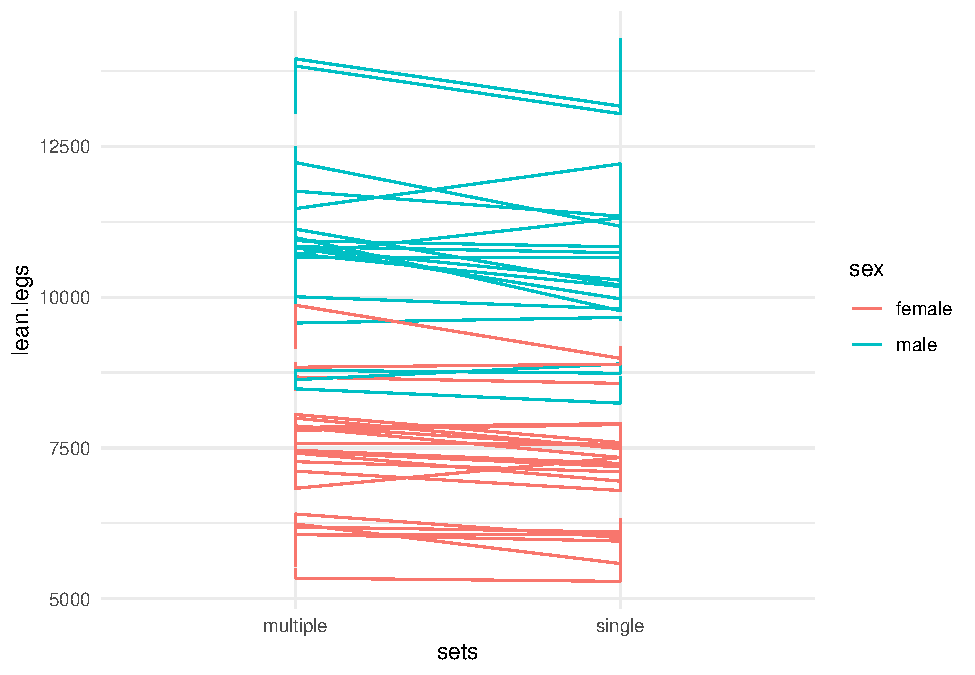
\includegraphics{_main_files/figure-latex/unnamed-chunk-9-1.pdf}

\hypertarget{styrke}{%
\subsubsection{Styrke}\label{styrke}}

Etter å ha justert for verdier ved baseline og kjønn så man at beinet som har gjennomført trening med enkeltsett hadde en signifikant lavere styrke etter avsluttet intervensjon enn beinet som hadde gjennomført trening med flersett. Fremgangen er målt i skalert motstand, som er motstand som en andel av maks. I skalert motstand hadde beinet med enkeltsett gjennomsnittlig 0.029(95\% CI) lavere verdier etter endt intervensjon enn beinet med flersett.

Gjennomsnittlig prosentvis endring i muskelstyrke fra baselinetesting til fullført intervensjon er vist i Tabell 3

\providecommand{\docline}[3]{\noalign{\global\setlength{\arrayrulewidth}{#1}}\arrayrulecolor[HTML]{#2}\cline{#3}}

\setlength{\tabcolsep}{2pt}

\renewcommand*{\arraystretch}{1.5}

\begin{longtable}[c]{|p{0.96in}|p{2.82in}}



\hhline{>{\arrayrulecolor[HTML]{666666}\global\arrayrulewidth=2pt}->{\arrayrulecolor[HTML]{666666}\global\arrayrulewidth=2pt}-}

\multicolumn{1}{!{\color[HTML]{000000}\vrule width 0pt}>{\raggedright}p{\dimexpr 0.96in+0\tabcolsep+0\arrayrulewidth}}{\fontsize{11}{11}\selectfont{\textcolor[HTML]{000000}{\global\setmainfont{Helvetica}{\ }}}} & \multicolumn{1}{!{\color[HTML]{000000}\vrule width 0pt}>{\raggedright}p{\dimexpr 2.82in+0\tabcolsep+0\arrayrulewidth}!{\color[HTML]{000000}\vrule width 0pt}}{\fontsize{11}{11}\selectfont{\textcolor[HTML]{000000}{\global\setmainfont{Helvetica}{Tabell\ 3\ -\ Økning\ beinstyrke\ i\ prosent}}}} \\

\noalign{\global\setlength{\arrayrulewidth}{2pt}}\arrayrulecolor[HTML]{666666}\cline{1-2}

\endfirsthead

\hhline{>{\arrayrulecolor[HTML]{666666}\global\arrayrulewidth=2pt}->{\arrayrulecolor[HTML]{666666}\global\arrayrulewidth=2pt}-}

\multicolumn{1}{!{\color[HTML]{000000}\vrule width 0pt}>{\raggedright}p{\dimexpr 0.96in+0\tabcolsep+0\arrayrulewidth}}{\fontsize{11}{11}\selectfont{\textcolor[HTML]{000000}{\global\setmainfont{Helvetica}{\ }}}} & \multicolumn{1}{!{\color[HTML]{000000}\vrule width 0pt}>{\raggedright}p{\dimexpr 2.82in+0\tabcolsep+0\arrayrulewidth}!{\color[HTML]{000000}\vrule width 0pt}}{\fontsize{11}{11}\selectfont{\textcolor[HTML]{000000}{\global\setmainfont{Helvetica}{Tabell\ 3\ -\ Økning\ beinstyrke\ i\ prosent}}}} \\

\noalign{\global\setlength{\arrayrulewidth}{2pt}}\arrayrulecolor[HTML]{666666}\cline{1-2}\endhead



\multicolumn{2}{!{\color[HTML]{FFFFFF}\vrule width 0pt}>{\raggedright}p{\dimexpr 3.77in+2\tabcolsep+1\arrayrulewidth}!{\color[HTML]{FFFFFF}\vrule width 0pt}}{\fontsize{11}{11}\selectfont{\textcolor[HTML]{000000}{\global\setmainfont{Helvetica}{Gjennomsnittlig\ prosentvis\ endring(SD),\ fra\ pre\ til\ post}}}} \\

\endfoot



\multicolumn{1}{!{\color[HTML]{000000}\vrule width 0pt}>{\raggedright}p{\dimexpr 0.96in+0\tabcolsep+0\arrayrulewidth}}{\fontsize{11}{11}\selectfont{\textcolor[HTML]{000000}{\global\setmainfont{Helvetica}{Flersett}}}} & \multicolumn{1}{!{\color[HTML]{000000}\vrule width 0pt}>{\raggedright}p{\dimexpr 2.82in+0\tabcolsep+0\arrayrulewidth}!{\color[HTML]{000000}\vrule width 0pt}}{\fontsize{11}{11}\selectfont{\textcolor[HTML]{000000}{\global\setmainfont{Helvetica}{31(14.2)}}}} \\





\multicolumn{1}{!{\color[HTML]{000000}\vrule width 0pt}>{\raggedright}p{\dimexpr 0.96in+0\tabcolsep+0\arrayrulewidth}}{\fontsize{11}{11}\selectfont{\textcolor[HTML]{000000}{\global\setmainfont{Helvetica}{Enkeltsett}}}} & \multicolumn{1}{!{\color[HTML]{000000}\vrule width 0pt}>{\raggedright}p{\dimexpr 2.82in+0\tabcolsep+0\arrayrulewidth}!{\color[HTML]{000000}\vrule width 0pt}}{\fontsize{11}{11}\selectfont{\textcolor[HTML]{000000}{\global\setmainfont{Helvetica}{24.5(12.9)}}}} \\

\noalign{\global\setlength{\arrayrulewidth}{2pt}}\arrayrulecolor[HTML]{666666}\cline{1-2}



\end{longtable}

.

\hypertarget{konklusjon}{%
\section{Konklusjon}\label{konklusjon}}

Fra baseline til etter intervensjonen var avsluttet var det en signifikant forskjell i fremgangen i beinet som gjennomførte trening med flersett sammenlignet med beinet som gjennomførte trening med enkeltsett. Dette gjaldt både mengden muskelmasse og muskelstyrke.

\hypertarget{kommentar}{%
\subsubsection{Kommentar}\label{kommentar}}

\hypertarget{kommentar-fra-daniel}{%
\paragraph{KOMMENTAR FRA DANIEL}\label{kommentar-fra-daniel}}

De samme deltakerne gjennomførte begge protokoller. Hva betyr: 123,5 gram mer(SD 55.17, 95\% CI)? Når du lager resultatene mer fullstendig, husk å trekke inferens på forskjell mellom treningsprotokoller og bruk deskriptiv statistikk på resterende data. Se og generell feedback på github (IDR4000-2021)

  \bibliography{book.bib,packages.bib}

\end{document}
